\subsubsection{NodeJs vs Apache PHP benchmark}

Tất cả các bài so sánh đều được thực hiện trong điều kiện:
\begin{framed}
	\begin{itemize}
		\item Server Apache 2.2.22
		\item Apache Bench 2.3
		\item Node.js v0.8.12
		\item Laptop: 
		
		\begin{itemize}
			\item Ubuntu: Release 12.04(precise) 32-bit
			\item KernelLinux 3.2.0-38-generic-pae
			\item GNOME 3.4.2
		\end{itemize}		

		\item Hardware:
		\begin{itemize}
			\item Memory: 3.8 GB
			\item Processor: IntelCore i3-2330M CPU @ 2.20GHz x 4
		\end{itemize}
	\end{itemize}
\end{framed}
	
	Chương trình này có $2$ tùy chọn quan trọng là -n số yêu cầu và -c số lượng yêu cầu đồng thời và cuối cùng là url.\\
Test với Node.js: \\
	\begin{center}
		\fbox{\texttt{/usr/bin/ab -n 100000 -c 1000 http://localhost:8080/}}
	\end{center}

Test với Apache:
	\begin{center}
		\fbox{\texttt{/usr/bin/ab -n 100000 -c 1000 http://localhost/}}
	\end{center}


\subsubsection*{Test với chương trình HelloWorld}
Chương trình đơn giản dùng để test với node.js server và Apache:\\
\texttt{hello.js}
	\begin{framed}
		\inputminted[tabsize=4,linenos=true]{javascript}{hello.js}
	\end{framed}

\texttt{index.php}
	\begin{framed}
		\inputminted[tabsize=4,linenos=true]{php}{index.php}
	\end{framed}

%========== Kết quả test HelloWorld ===============
Sau quá trình test ta thu được các kết quả dưới bảng sau:(Thời gian tính theo đơn vị giây)\\
\textbf{$100,000$ yêu cầu, $1000$ yêu cầu đồng thời} \\
	\begin{tabular}{|c|c|c|c|c|c|}
		\hline
		x & 1 & 2 & 3 & 4 & 5 \\
		\hline
		Apache & 25.972 & 27.908 & 26.708 & 29.893 & 25.980 \\
		\hline
		NodeJs & 14.467 & 14.643 & 15.854 & 16.724 & 14.389
		\\ \hline
	\end{tabular}
\newpage

Đồ thị minh họa:\\
	\begin{figure}[-h]
		\centering
		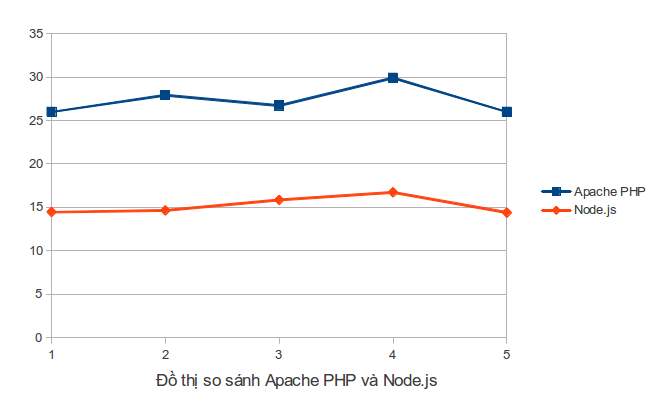
\includegraphics[scale=0.6]{1_1.png}
	\end{figure}

\subsection{Test với chương trình tính số PI}
	Chương trình sử dụng để test:\\
\texttt{testPI.js}
		\begin{framed}
			\inputminted[tabsize=4, linenos=true]{javascript}{testPI.js}
		\end{framed}

\texttt{testPI.php}
		\begin{framed}
			\inputminted[tabsize=4, linenos=true]{php}{testPi.php}
		\end{framed}

%========== Kết quả tính toán số PI ===============
Sau quá trình test ta thu được kết quả trong bảng dưới đây:	\\
	\begin{tabular}{|c|c|c|c|c|c|}
		\hline
		x & 1 & 2 & 3 & 4 & 5 \\
		\hline
		Apache & 26.001 & 27.134 & 26.801 & 28.201 & 27.040 \\
		\hline
		NodeJs & 3.181 & 3.198 & 3.423 & 4.214 & 3.426
		\\ \hline
	\end{tabular}


Đồ thị minh họa:\\
	\begin{figure}[-h]
		\centering
		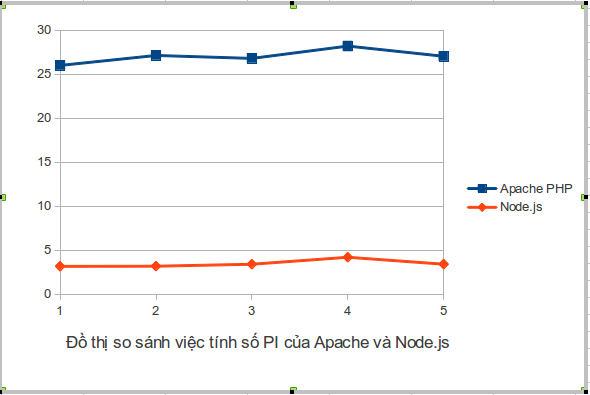
\includegraphics[scale=0.6]{1_2.png}
	\end{figure}

